
Code at \url{https://github.com/cedrict/fieldstone/tree/master/python_codes/fieldstone_43}

The following five experiments are pure-advection experiments. As such the Peclet number
is infinite and the $\gamma$ value of the SUPG algorithm as shown in Section~\ref{ss:supg} tends to 1
and the $\tau$ parameter is simply $h/2 |\vec\upnu| p$ (where $p$ is the order of the shape function polynomials).

Note that although the code can deal with linear elements, all results hereafter are obtained with quadratic elements (unless specified otherwise). 

%...........................................................................................
\paragraph{Experiment 1}

This benchmark originates in \cite{dohu03}. It is also carried out in \cite{bepo10}.
It considers the advection of a product-cosine hill
in a prescribed velocity field. The initial temperature is:
\begin{equation}
T_0(x,y)=
\left\{
\begin{array}{cc}
\frac{1}{4}
\left(1+\cos \pi\frac{x-x_c}{\sigma}\right)
\left(1+\cos \pi\frac{y-y_c}{\sigma}\right)
& \text{if } (x-x_c)^2+(y-y_c)^2\leq \sigma^2 \\
0 & \text{otherwise}
\end{array}
\right.
\end{equation}
The boundary conditions are $T(x,y)=0$ on all four sides of the unit square domain. 
In what follows we set $x_c=y_c=1/6$ and $\sigma=0.2$.  
The velocity field is analytically prescribed: $\vec\upnu=(-(y-y_c),+(x-x_c))$.
Resolution is set to $30\times30$ quadratic elements.

In what follows we test the time integration scheme by setting $\alpha_T=1$ (fully implicit formulation), $\alpha=0$ (fully explicit formulation) and $\alpha_T=1/2$ (Crank-Nicolson).  
In the book Donea \& Huerta set the timestep is set to $\delta t=2\pi/200$ which corresponds to a CFL number of approximately 0.666. If we want to be able to run this experiment at higher 
resolution we need to adapt the timestep to the mesh size (CFL criterion). We therefore set the CFL number to 0.5 and compute $\delta t$ accordingly (see Section~\ref{ss:cfl}).  
The density and heat capacity values are set to 1. We monitor the minimum and maximum value of the temperature field, as well as the total thermal energy $E_T$ in the 
system during the full rotation:
\[
E_T=\int_\Omega \rho_0 C_p T dV = \int_\Omega T dV = |\Omega| \langle T \rangle 
\qquad
\text{where}
\qquad
\langle T \rangle = \frac{1}{|\Omega|} \int_\Omega T dV
\]
The time evolution of the temperature with the Crank-Nicolson algorithm is shown hereunder:
\begin{center}
a)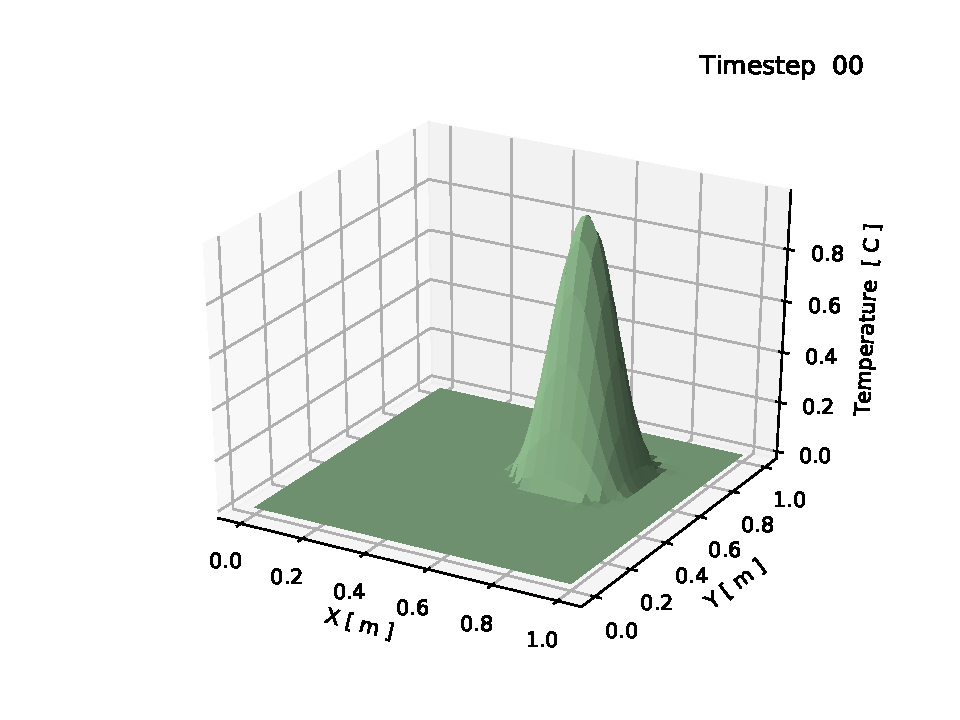
\includegraphics[width=4.8cm]{python_codes/fieldstone_43/results/experiment1/crni/solution_0000.pdf}
b)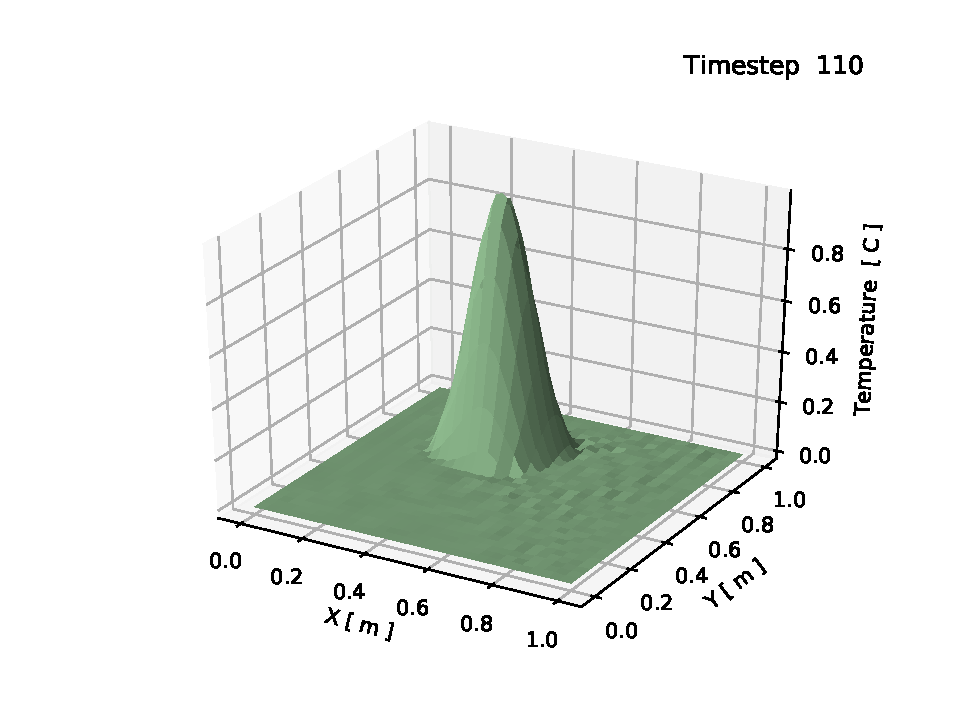
\includegraphics[width=4.8cm]{python_codes/fieldstone_43/results/experiment1/crni/solution_0110.pdf}
c)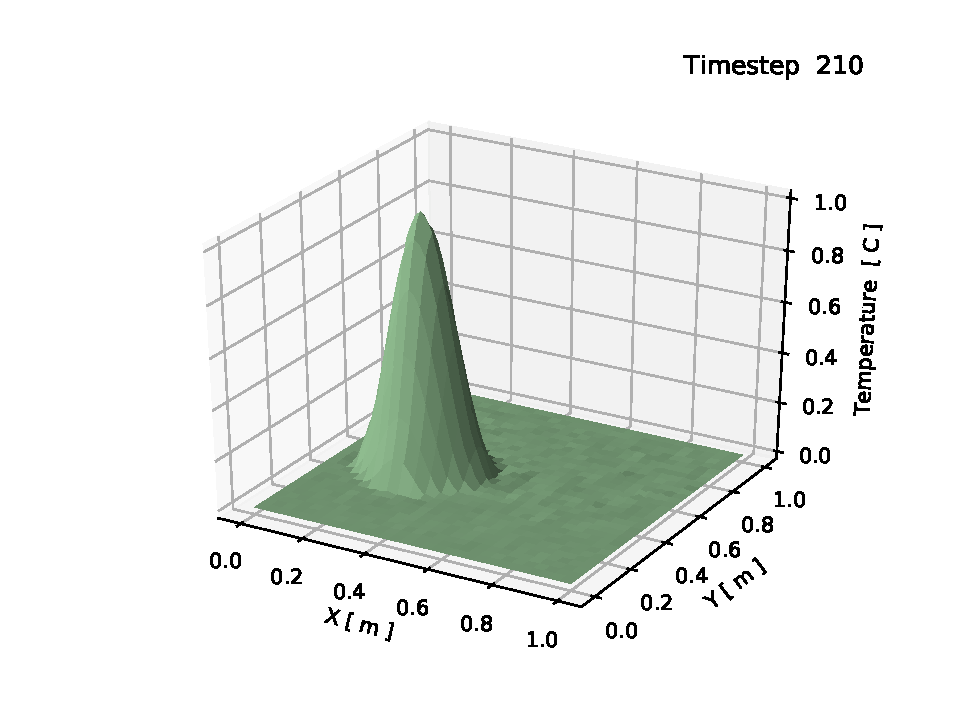
\includegraphics[width=4.8cm]{python_codes/fieldstone_43/results/experiment1/crni/solution_0210.pdf}
d)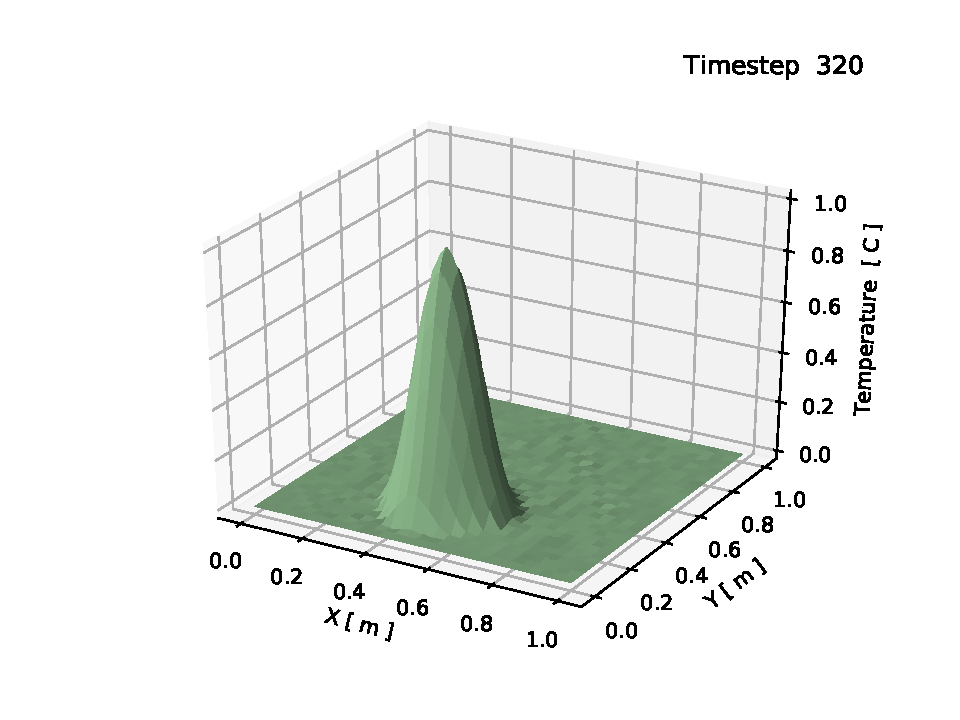
\includegraphics[width=4.8cm]{python_codes/fieldstone_43/results/experiment1/crni/solution_0320.pdf}
e)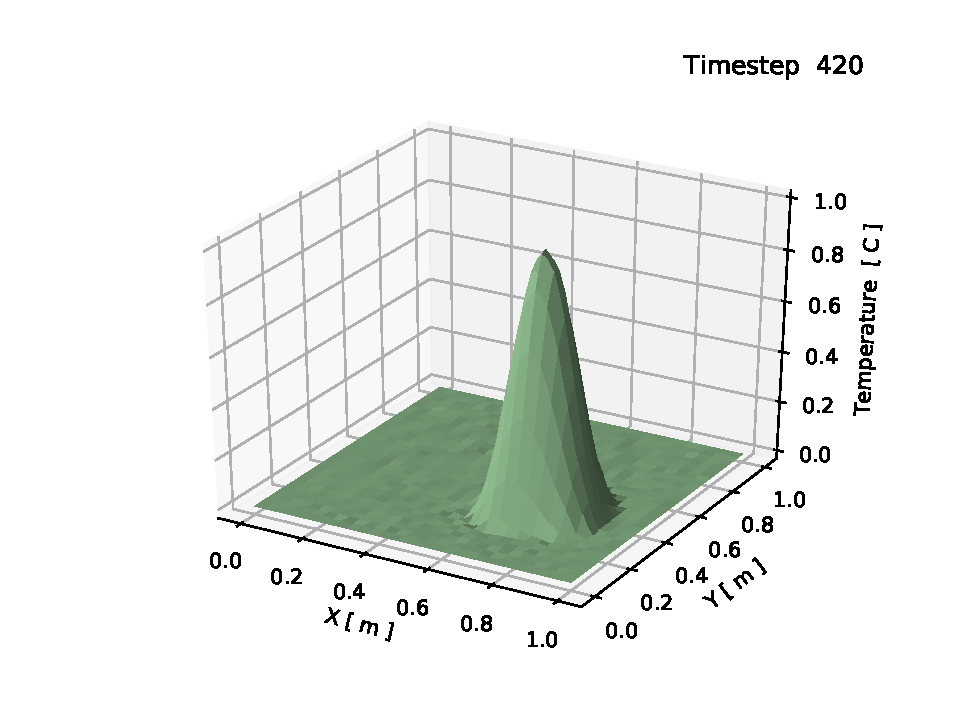
\includegraphics[width=4.8cm]{python_codes/fieldstone_43/results/experiment1/crni/solution_0420.pdf}
f)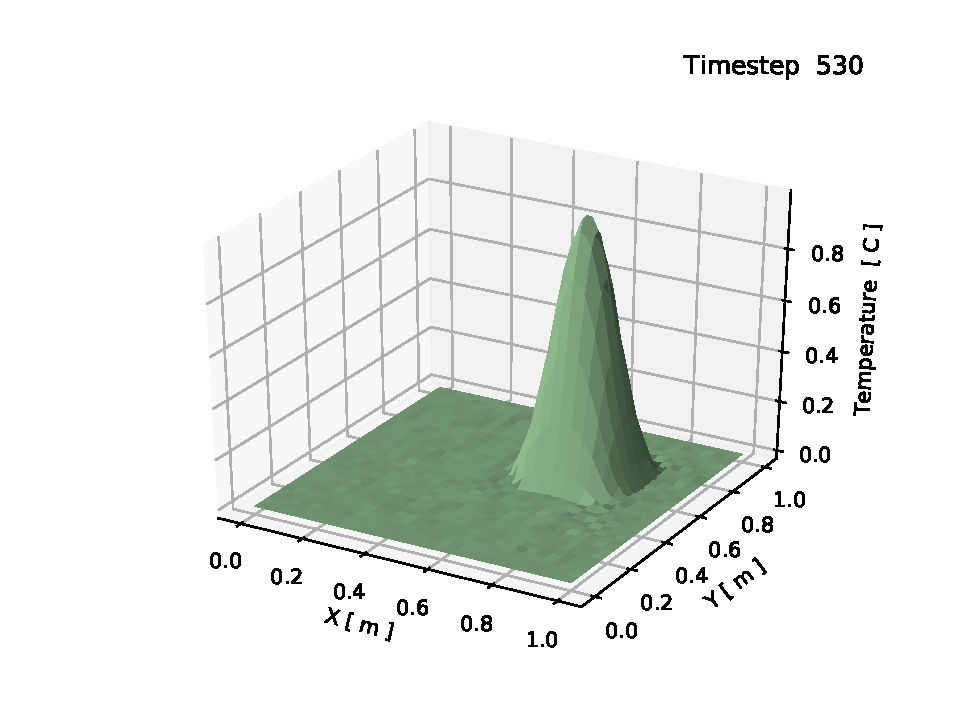
\includegraphics[width=4.8cm]{python_codes/fieldstone_43/results/experiment1/crni/solution_0530.pdf}\\
{\captionfont a,b,c,d,e,f) Temperature field throughout the rotation.} 
\end{center}

\vspace{.4cm}

Turning now to the statistics, we plot $\min(T)$, $\max(T)$ and $E_T$ as a function of time:
\begin{center}
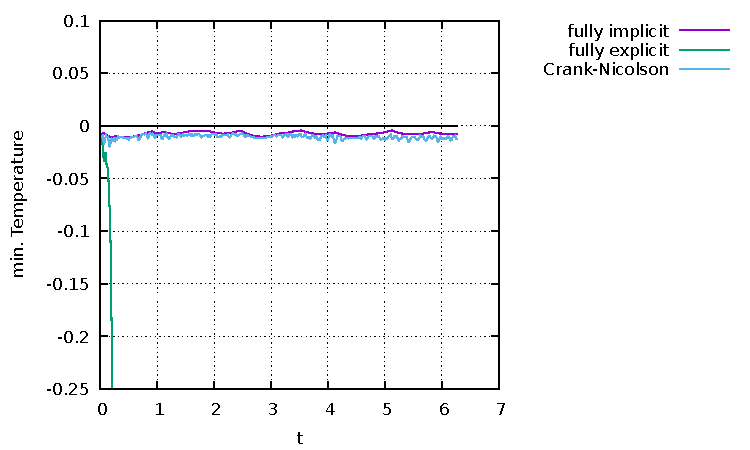
\includegraphics[width=5cm]{python_codes/fieldstone_43/results/experiment1/Tmin.pdf}
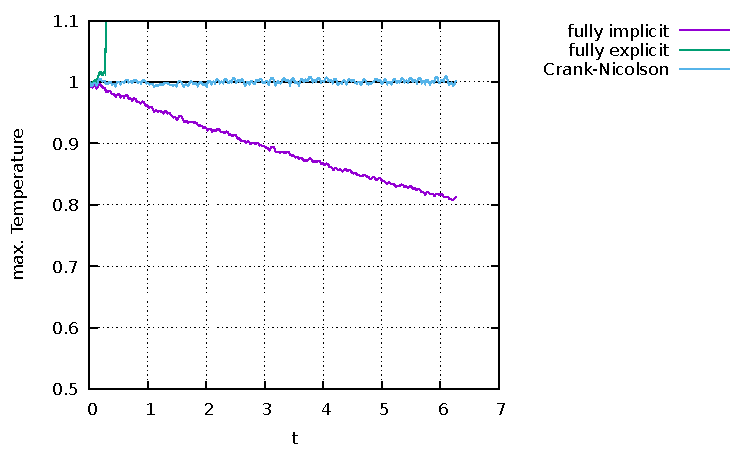
\includegraphics[width=5cm]{python_codes/fieldstone_43/results/experiment1/Tmax.pdf}
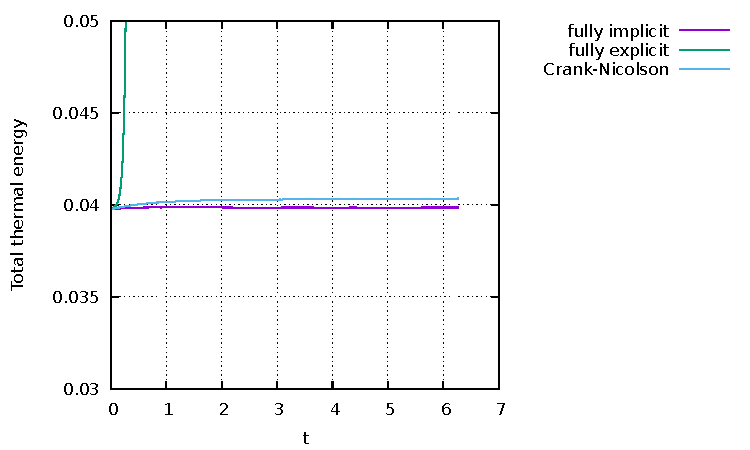
\includegraphics[width=5cm]{python_codes/fieldstone_43/results/experiment1/ET.pdf}\\
{\captionfont Time evolution of the min and max temperature and the total energy}
\end{center}
The conclusions are clear: the explicit method diverges quickly and is unusable. The fully implicit and Crank-Nicolson 
method yield similar energy conservation but the fully-implicit showcases a clear loss in maximum temperature.

$\bigtriangleup$ Finally we can run the experiment (still a $2\pi$ rotation) 
with three different time steps ($\delta t=2\pi/30,2\pi/60,2\pi/120$) 
and we recover very similar results to those presented in \cite{dohu03}:
\begin{center}
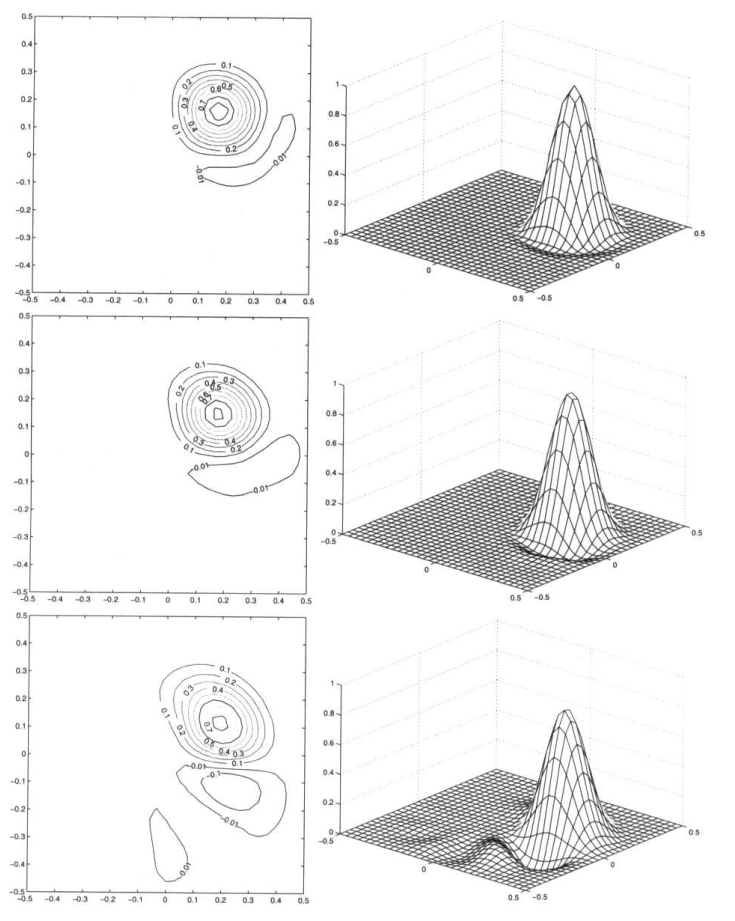
\includegraphics[height=8cm]{python_codes/fieldstone_43/results/experiment1/dohu03}
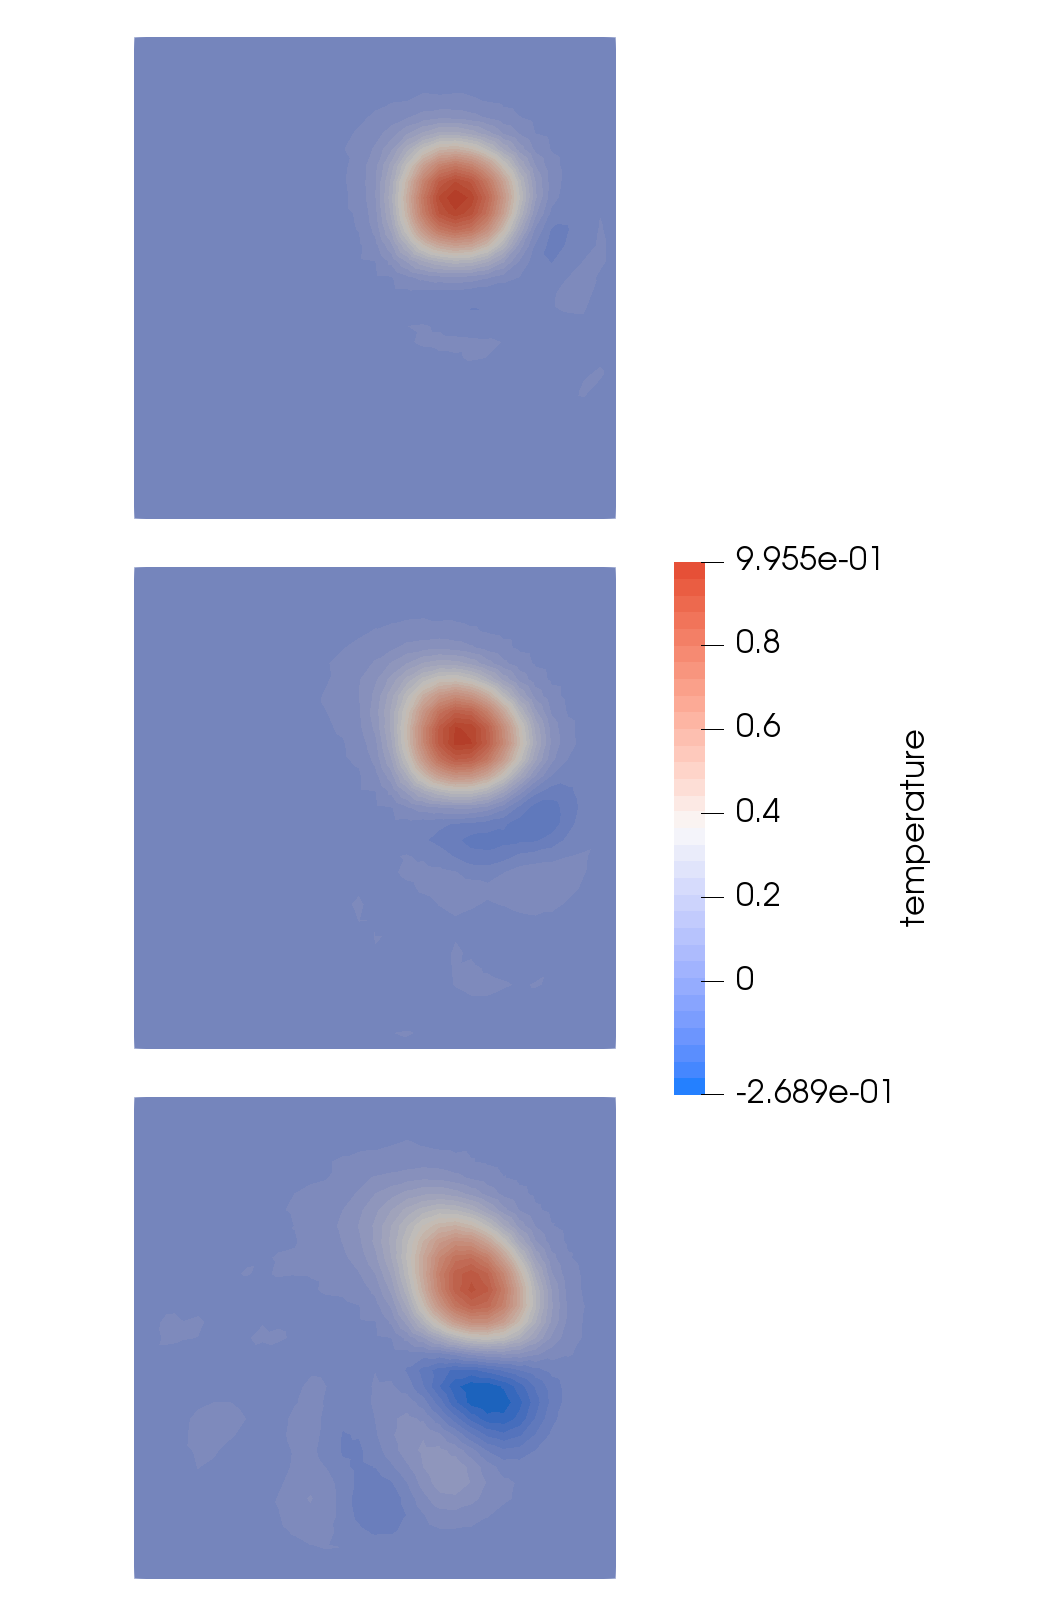
\includegraphics[height=8cm]{python_codes/fieldstone_43/results/experiment1/temps_30_60_120}\\
{\captionfont From top to bottom: $\delta t=2\pi/120,2\pi/60,2\pi/30$ with Crank-Nicolson. Left panel is taken from donea \& Huerta \cite{dohu03}. Results obtained with linear elements.}
\end{center}



$\bigtriangleup$ 
I have also implemented BDF1,2,3,4,5  (see Section~\ref{ss:hte_fem}). 
BDF2 outperforms BDF1 and is comparable to Crank-Nicolson. 
For reasons unknown to me, the BDF3 diverges after 100 time steps. So do 
BDF4 and BDF5 after even less timesteps. In the following picture the temperature is shown for 
BDF1,2,3 and Crank-Nicolson after a full rotation.

\begin{center}
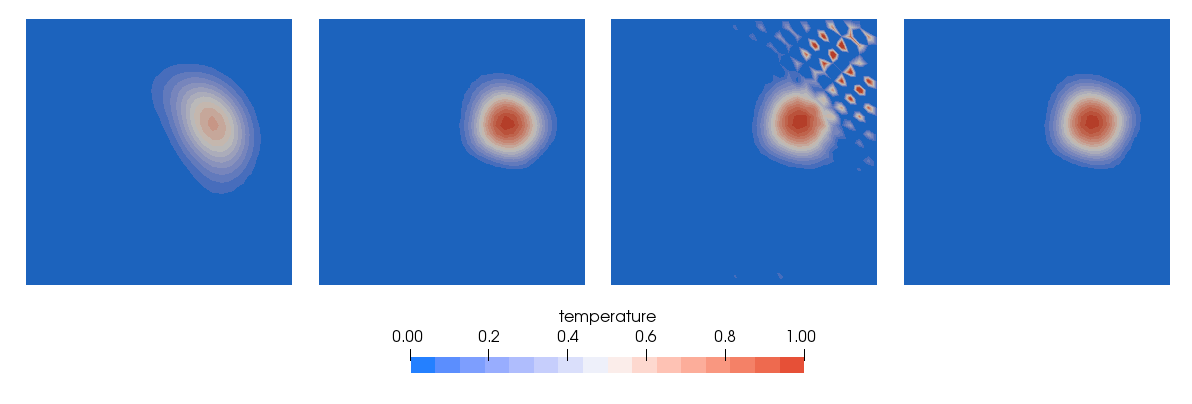
\includegraphics[width=15cm]{python_codes/fieldstone_43/results/experiment1/Tbdf123crni.png}\\
{\captionfont Left to right: BDF1 (i.e. implicit euler), BDF2, BDF3, Crank-Nicolson}
\end{center}

I now turn to another aspect of this problem: what is the effect of the SUPG stabilisation 
scheme on the solution? In what follows Crank-Nicolson is used. 

\begin{center}
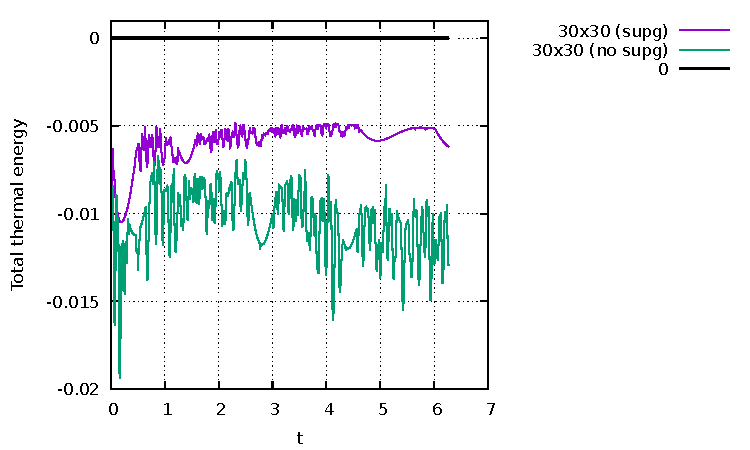
\includegraphics[width=6cm]{python_codes/fieldstone_43/results/experiment1/Tmin_supg}
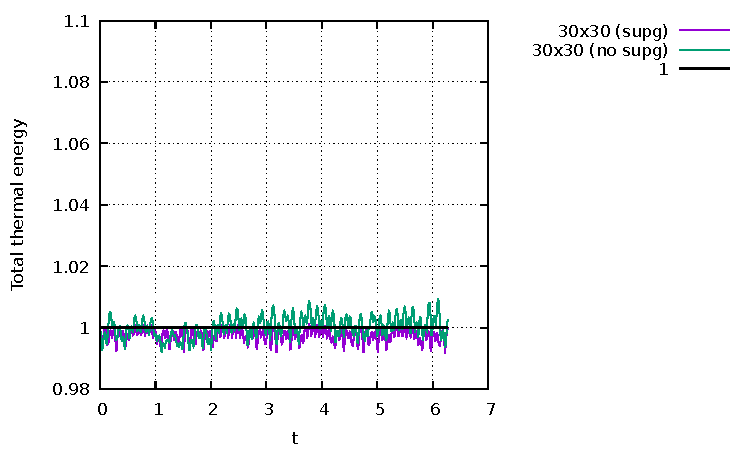
\includegraphics[width=6cm]{python_codes/fieldstone_43/results/experiment1/Tmax_supg}\\
{\captionfont Time evolution of min/max temperature with and without SUPG.} 
\end{center}

%...........................................................................................
\paragraph{Experiment 2}

This setup is inspired by the one in the ASPECT manual. The cone of the previous 
experiment is now replaced by three 'objects': a Zalesak disk \ref{zale79}, a sharp cone and a truncated cosine hill:

\begin{lstlisting}
for i in range(0,NV):
    xi=x[i]
    yi=y[i]
    if np.sqrt(xi**2+(yi-0.5)**2)<0.3 and (np.abs(xi)>=0.05 or yi>=0.7):
       T[i]=1
    if np.sqrt((x[i])**2+(y[i]+0.5)**2)<0.3:
       T[i]=1-np.sqrt((x[i])**2+(y[i]+0.5)**2)/0.3
    if np.sqrt((x[i]+0.5)**2+(y[i])**2)<0.3:
       T[i]=0.25*(1+np.cos(np.pi*np.sqrt((xi+0.5)**2+yi**2)/0.3))
\end{lstlisting}

The domain is $2\times2$, centered on the origin. The velocity is $\vec\upnu=(-y,x)$. Temperature 
is set to zero on all four sides.
For this experiment the CFL number is set to 0.5

\begin{center}
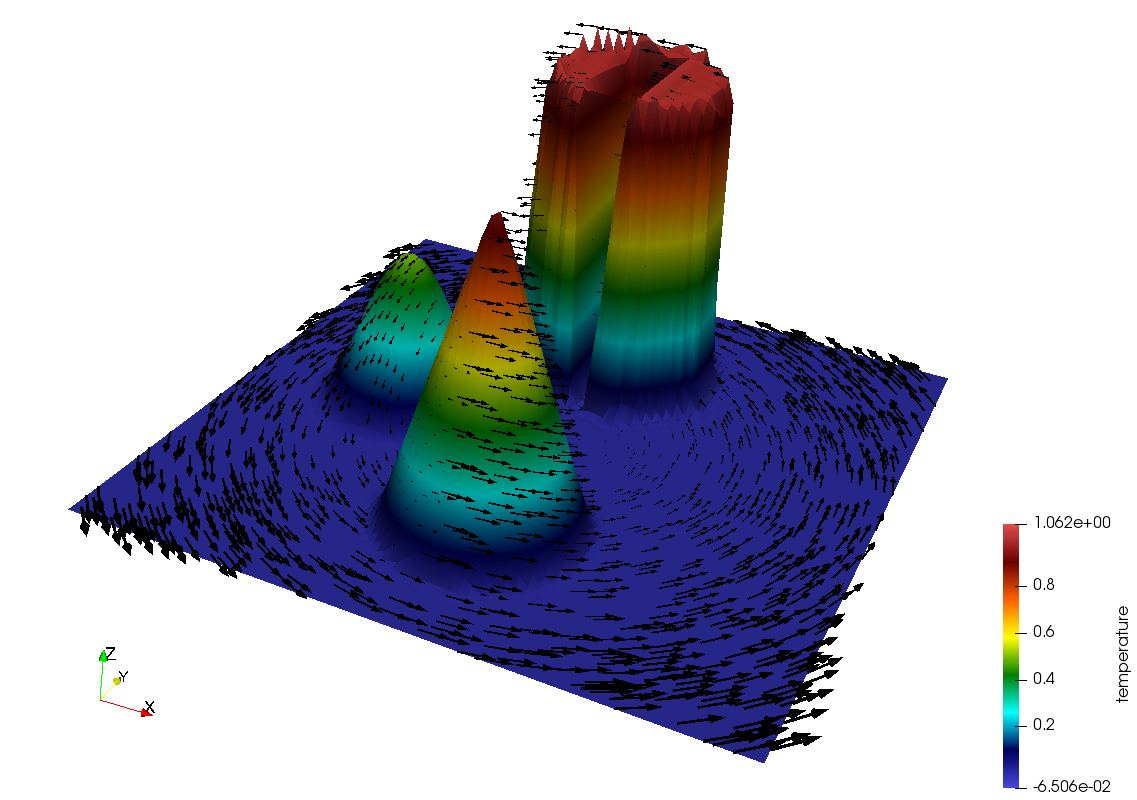
\includegraphics[width=8cm]{python_codes/fieldstone_43/results/experiment2/buildings}\\
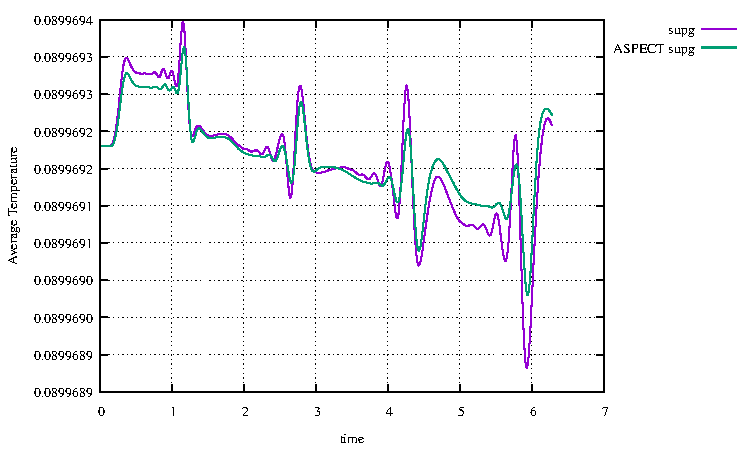
\includegraphics[width=7cm]{python_codes/fieldstone_43/results/experiment2/avrg_T}
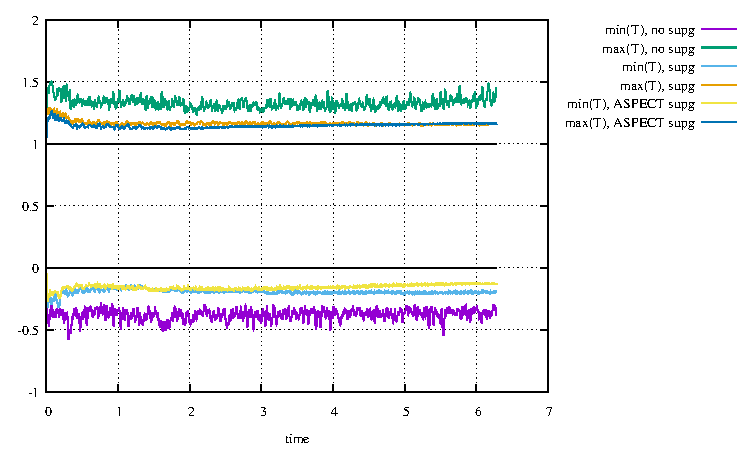
\includegraphics[width=7cm]{python_codes/fieldstone_43/results/experiment2/stats_T}
\end{center}

\begin{center}
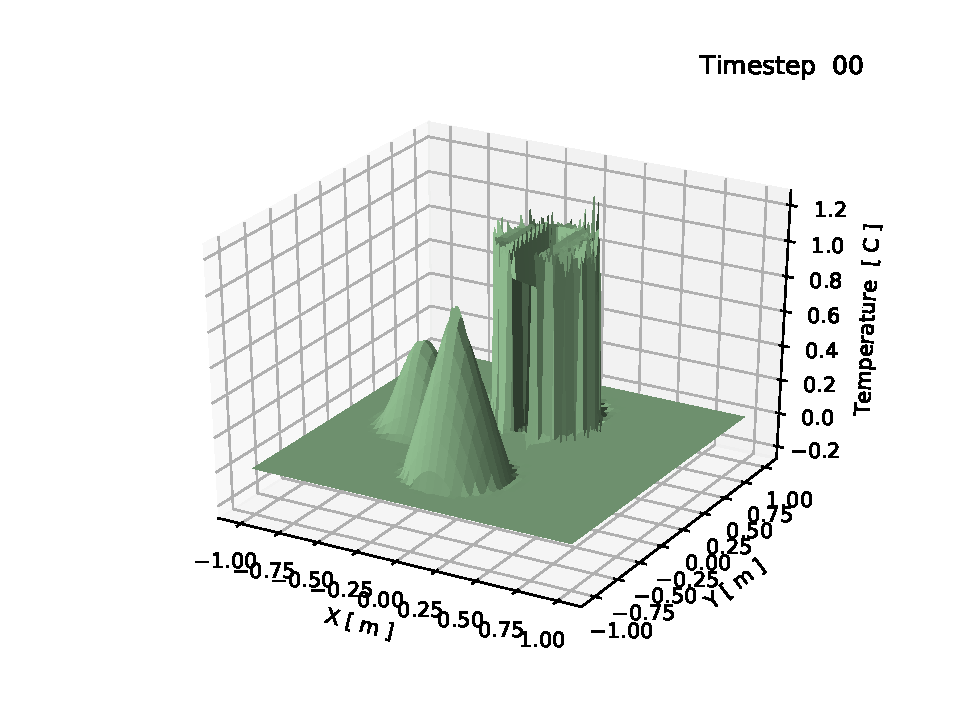
\includegraphics[width=3.2cm]{python_codes/fieldstone_43/results/experiment2/supg/solution_0000.pdf}
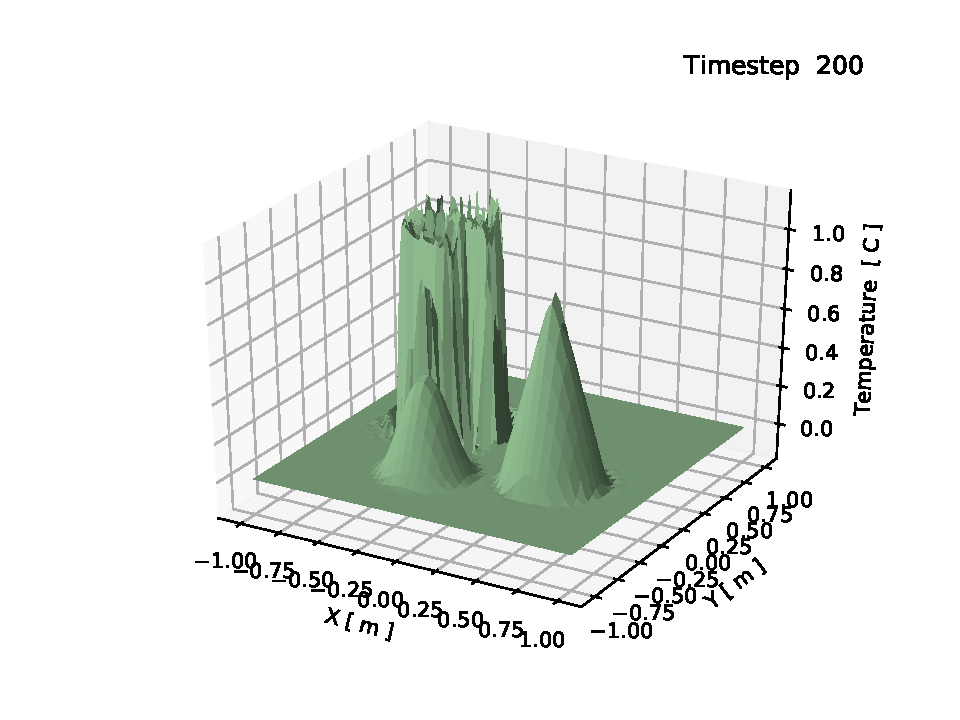
\includegraphics[width=3.2cm]{python_codes/fieldstone_43/results/experiment2/supg/solution_0200.pdf}
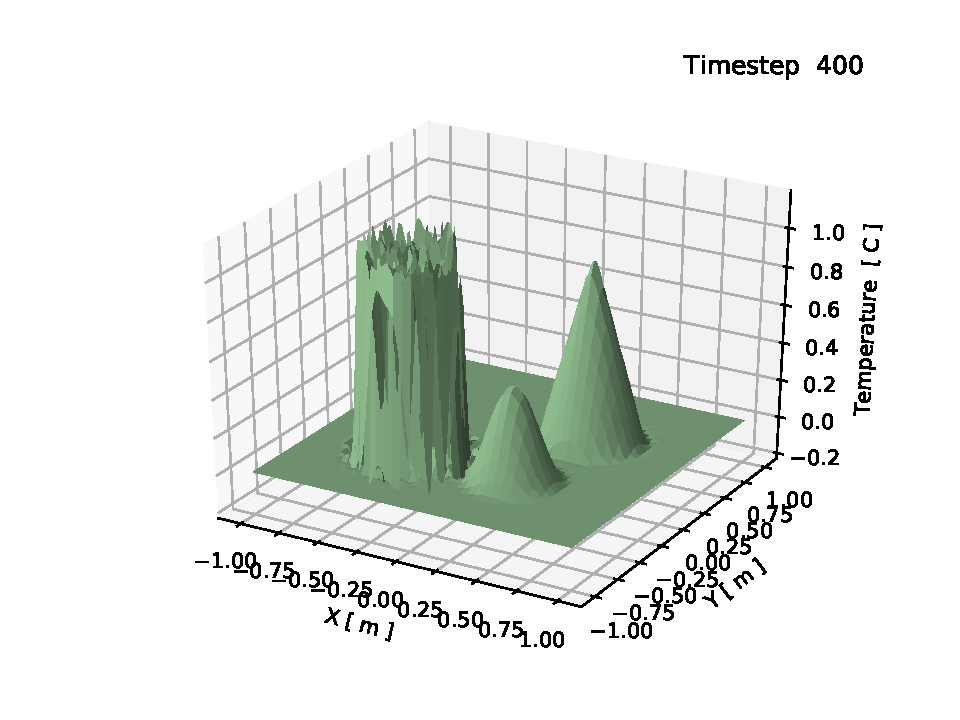
\includegraphics[width=3.2cm]{python_codes/fieldstone_43/results/experiment2/supg/solution_0400.pdf}
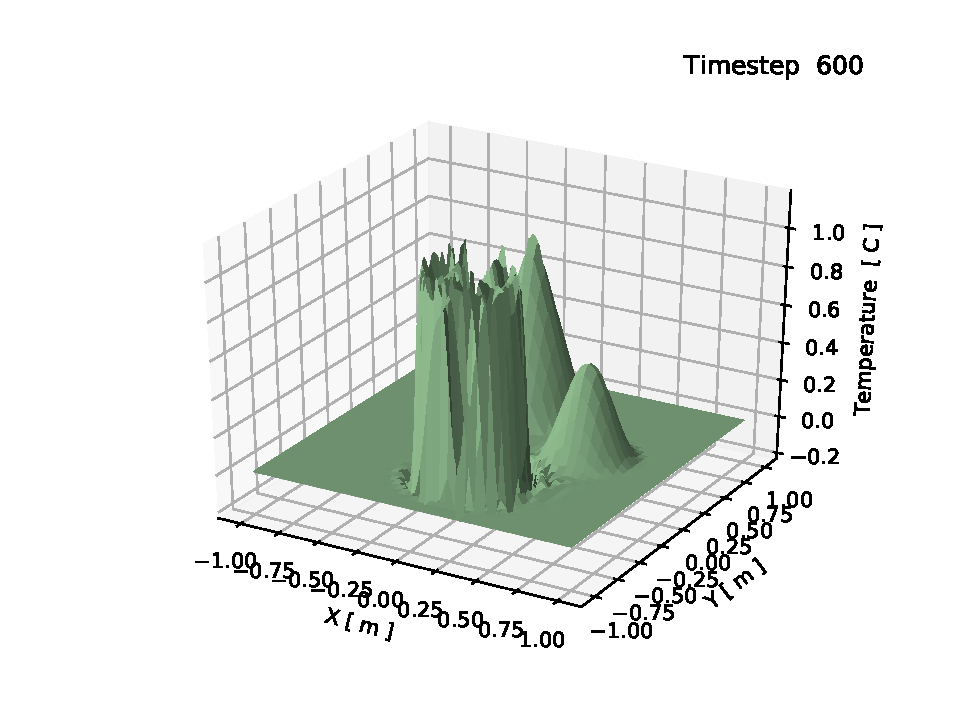
\includegraphics[width=3.2cm]{python_codes/fieldstone_43/results/experiment2/supg/solution_0600.pdf}\\
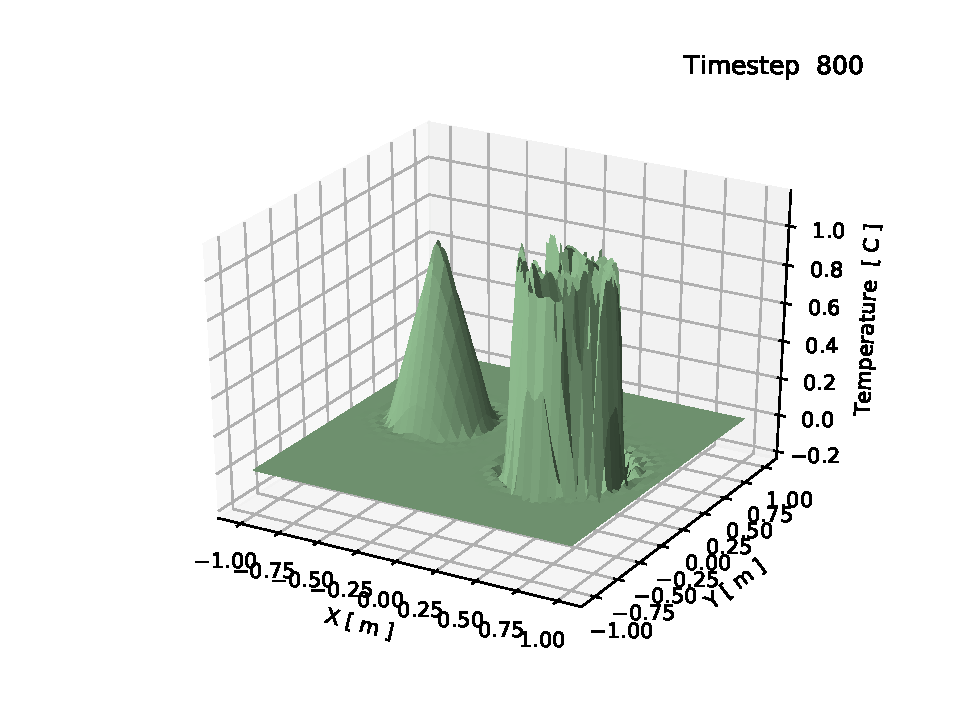
\includegraphics[width=3.2cm]{python_codes/fieldstone_43/results/experiment2/supg/solution_0800.pdf}
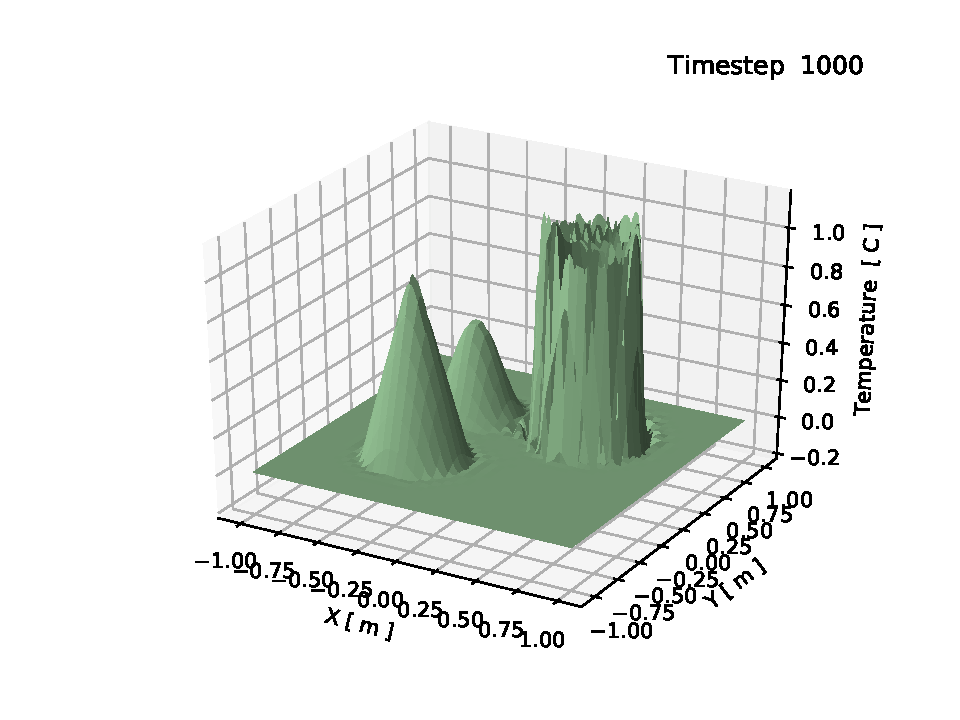
\includegraphics[width=3.2cm]{python_codes/fieldstone_43/results/experiment2/supg/solution_1000.pdf}
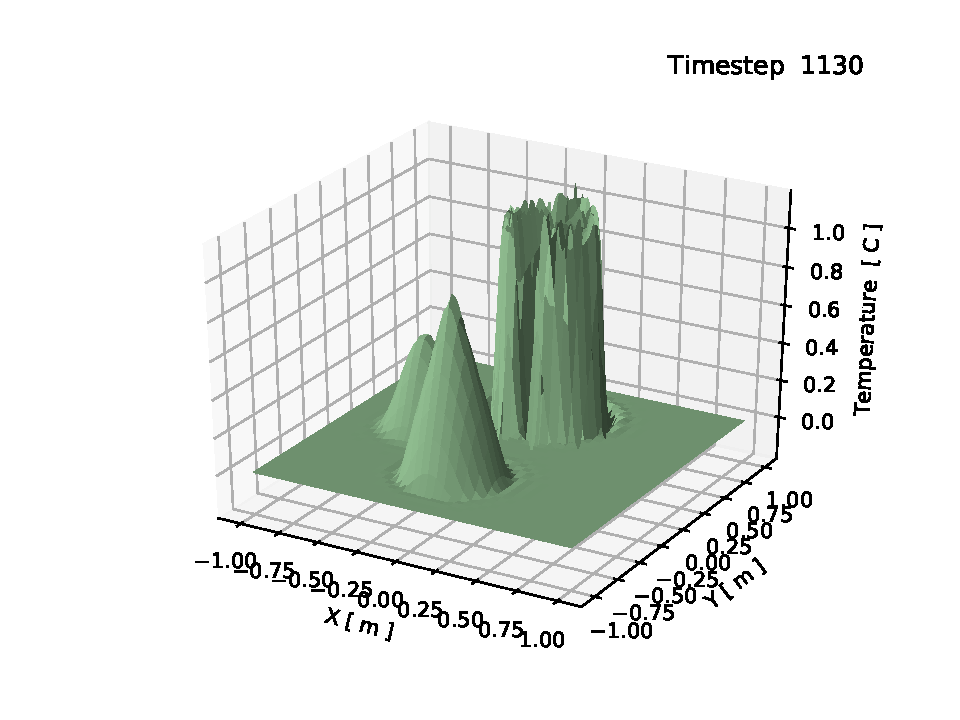
\includegraphics[width=3.2cm]{python_codes/fieldstone_43/results/experiment2/supg/solution_1130.pdf}\\
{\captionfont Time evolution of the temperature field with Crank-Nicolson, with SUPG.}
\end{center}


\begin{center}
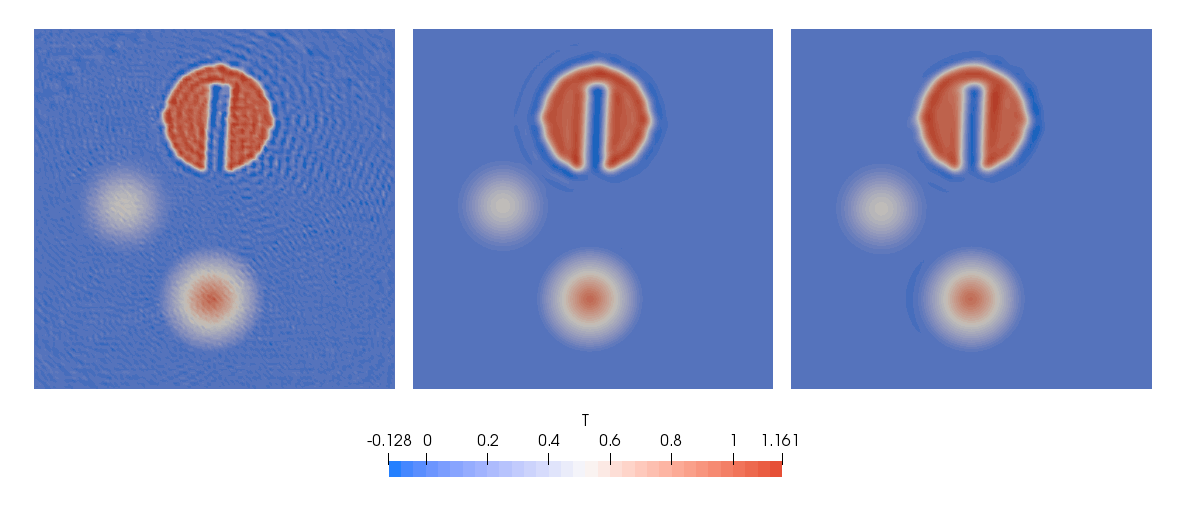
\includegraphics[width=15cm]{python_codes/fieldstone_43/results/experiment2/Temps}\\
{\captionfont Left: no SUPG; middle: with SUPG; right: ASPECT with SUPG}
\end{center}


%...........................................................................................
\paragraph{Experiment 3}

This experiment comes from Appendix A of Thieulot (2011) \cite{thie11}.
The unit segment is discretised by means of 64 elements, 
over which a unit velocity field is prescribed.
The discontinuity is initially
placed at x = 1/4 and after a time $t=0.5$, it is expected to have
reached the position $x=3/4$.
Temperature boundary conditions are $T=1$ on the left and $T=0$ on the right. 
Note that the simulation is actually carried out in 2D with a $1\times0.25$ domain 
discretised by means of $64\times16$ elements.
CFL number is set to 0.25

%\[
%\tau_{supg} = \frac{h}{2 d |\vec{\upnu}|} = \frac{\sqrt{2}/50}{2 \cdot 1 \cdot 1} = 0.01414
%\]

%\begin{center}
%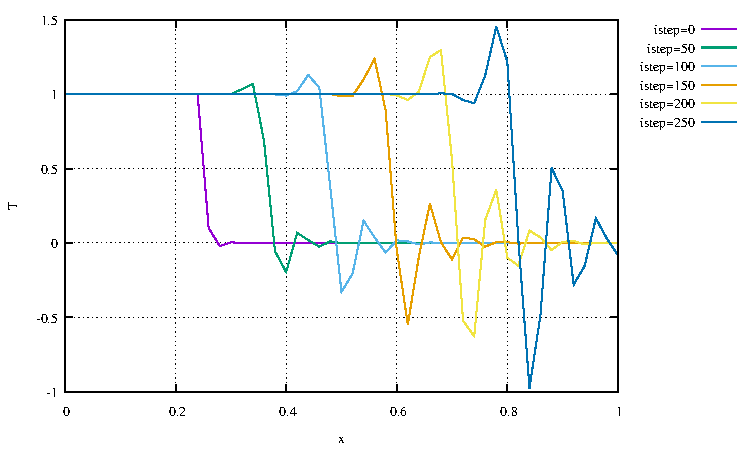
\includegraphics[width=8cm]{python_codes/fieldstone_43/results/experiment3/Q1/supg1/T.pdf}
%\includegraphics[width=6cm]{python_codes/fieldstone_43/results/experiment3/Q1/supg1/solution_0250.pdf}
%\end{center}


\[
\tau_{supg} = \frac{h}{2 d |\vec{\upnu}|} = \frac{\sqrt{2}/64}{2 \cdot 2 \cdot 1} = 0.005524
\]

\begin{center}
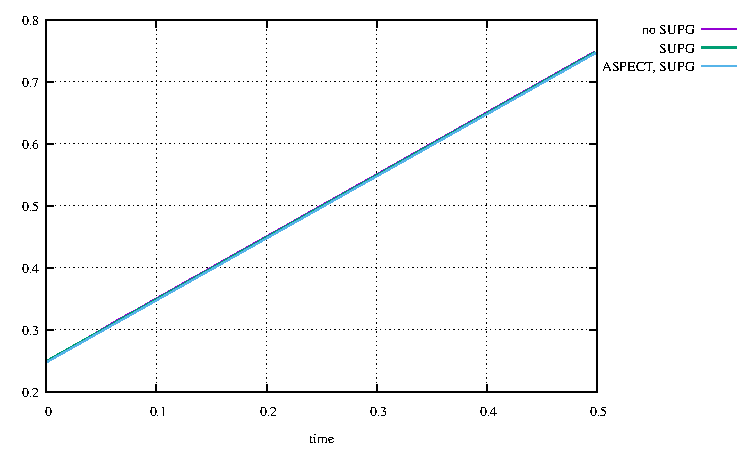
\includegraphics[width=5cm]{python_codes/fieldstone_43/results/experiment3/Q2/avrg_T.pdf}
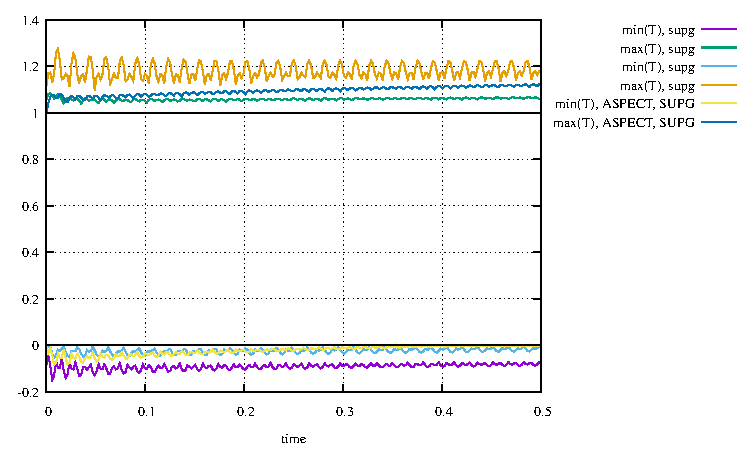
\includegraphics[width=5cm]{python_codes/fieldstone_43/results/experiment3/Q2/stats_T.pdf}
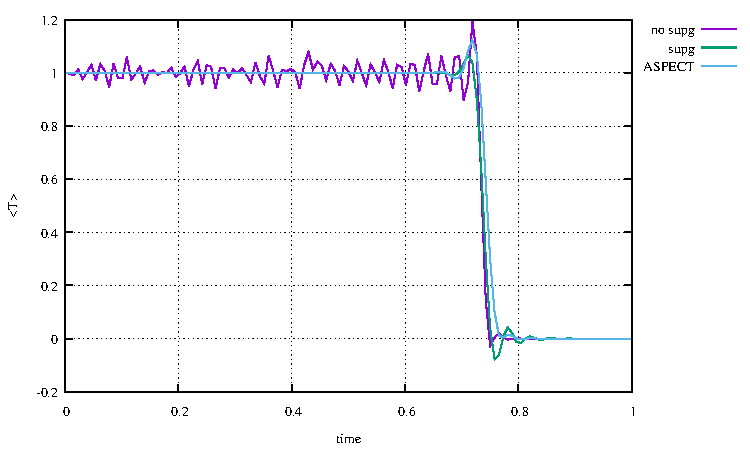
\includegraphics[width=5cm]{python_codes/fieldstone_43/results/experiment3/Q2/temperature.pdf}
\end{center}





%...........................................................................................
\paragraph{Experiment 4}

This experiment is somewhat similar to the one in fieldstone \ref{f65}.
The domain is a unit square, and the velocity is given by $\vec\upnu=(\cos \theta, \sin\theta)$ with $\theta=\pi/6$.
The temperature is prescribed on the left side only, i.e. $T=1$ for $x=0$, $y=[0,1]$ (corners included), and 
on the bottom (left corner excluded) with $T=0$. The other two sides are left free. Initial temperature is $T=0$.
The resolution is $10\times10$ and the CFL number is set to $C=10^{-1}$. The model is run up to $t=3$ (steady 
state is then reached). 

\begin{center}
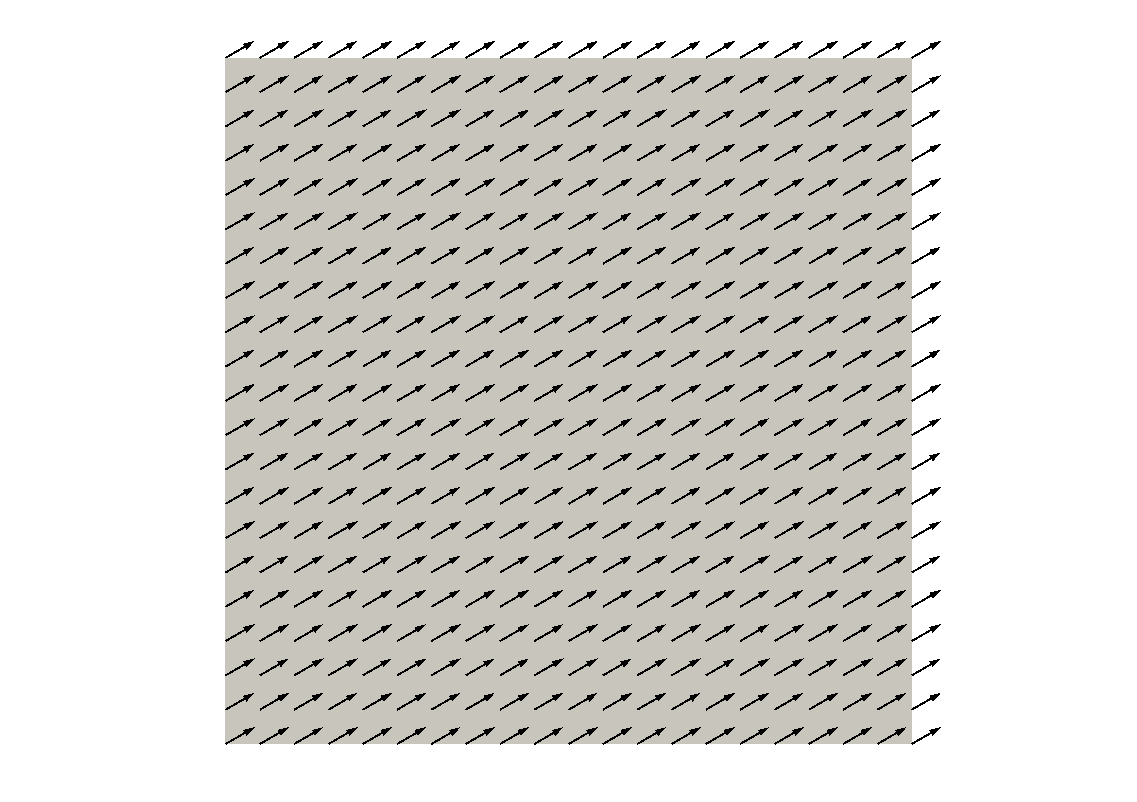
\includegraphics[width=5cm]{python_codes/fieldstone_43/results/experiment4/vel}
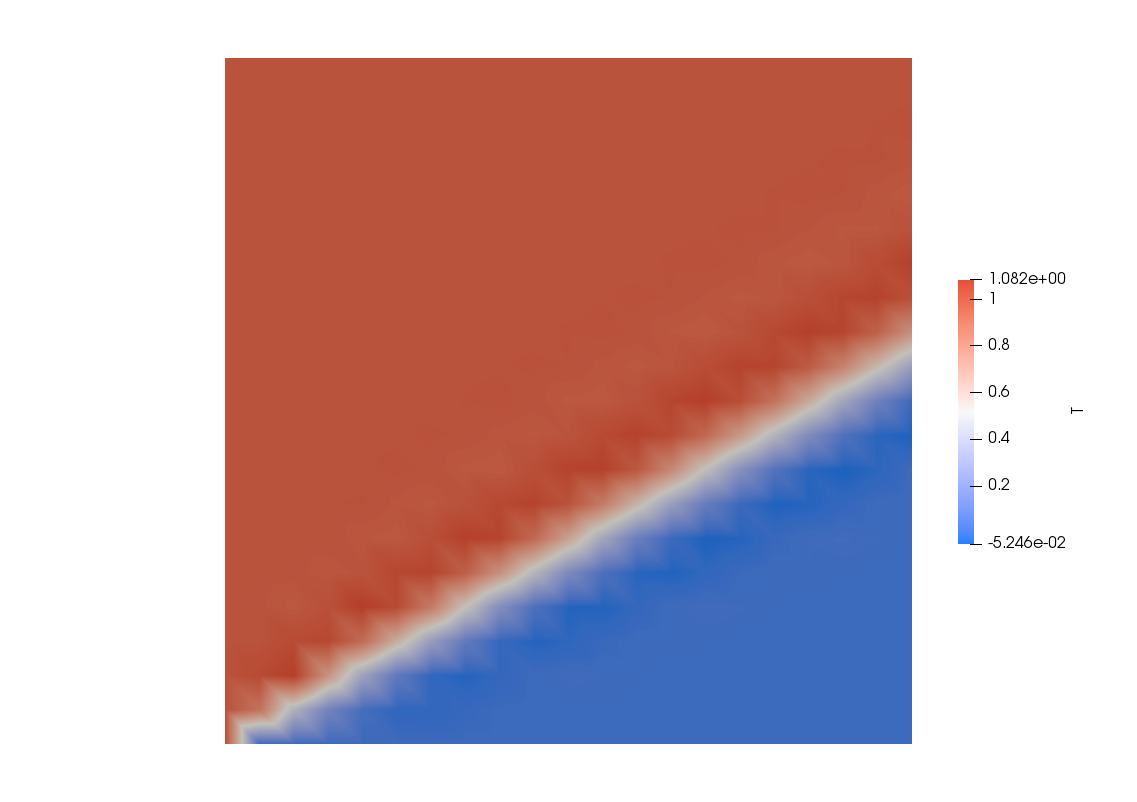
\includegraphics[width=5cm]{python_codes/fieldstone_43/results/experiment4/Tss}
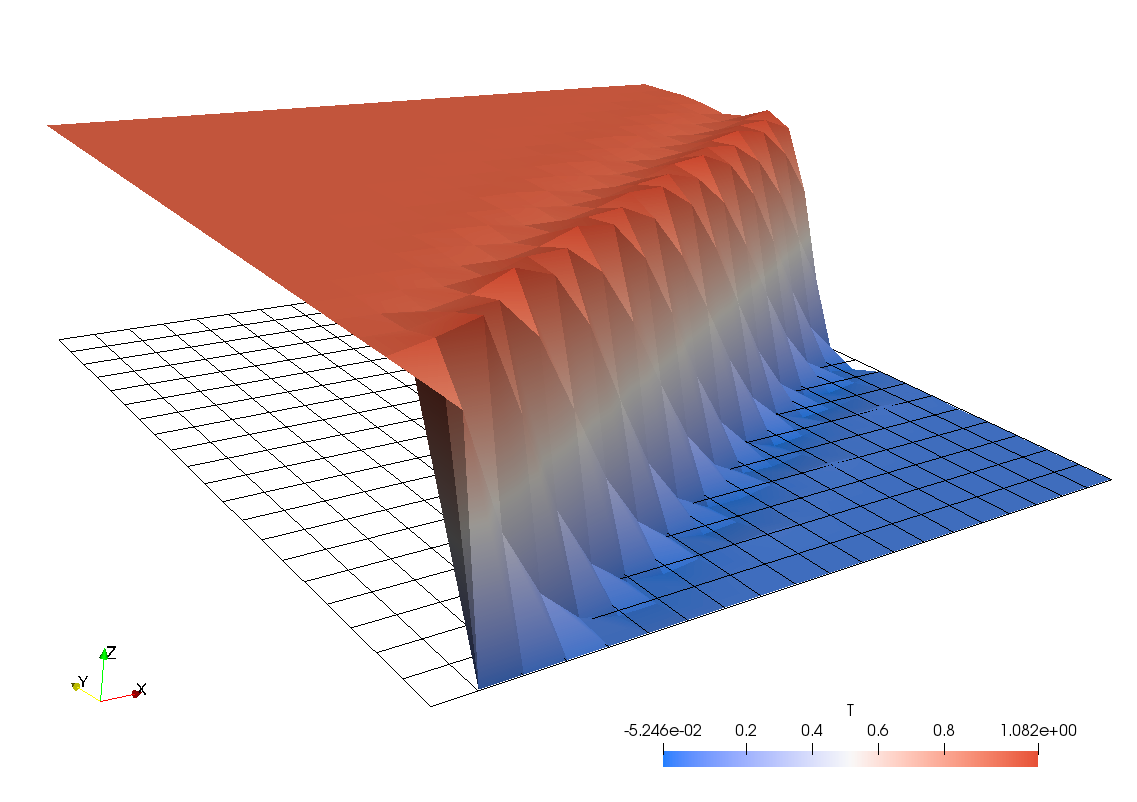
\includegraphics[width=5cm]{python_codes/fieldstone_43/results/experiment4/Tss3D}\\
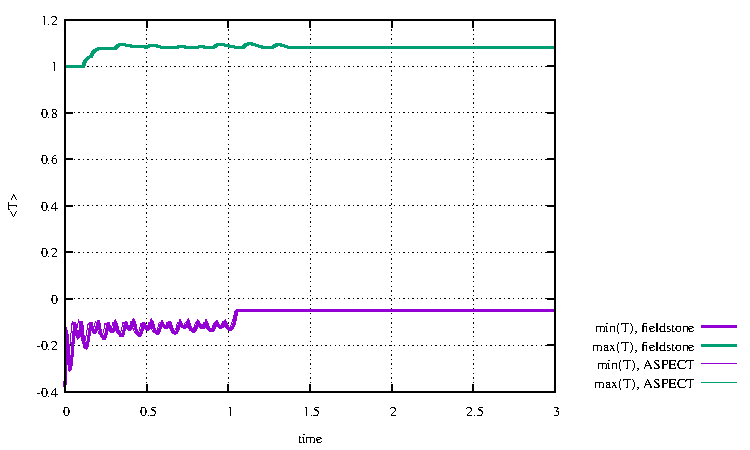
\includegraphics[width=7cm]{python_codes/fieldstone_43/results/experiment4/stats_T}
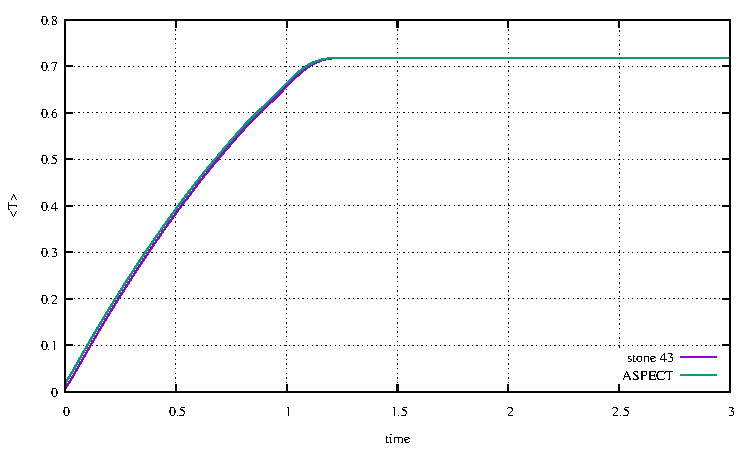
\includegraphics[width=7cm]{python_codes/fieldstone_43/results/experiment4/avrg_T}
\end{center}

%...........................................................................................
\paragraph{Experiment 5}

The domain is a unit square. The velocity field is given by $\vec\upnu=(y,1-x)$. Initial temperature is 
$T=0$. On left boundary $T=0$ is prescribed while at the bottom $T=0$ is prescribed if $x<1/3$ and $T=1$
otherwise. Resolution is $16\times16$ and the CFL number is set to $C=10^{-1}$. The model is run up to $t=4$ (steady
state is then reached).

\begin{center}
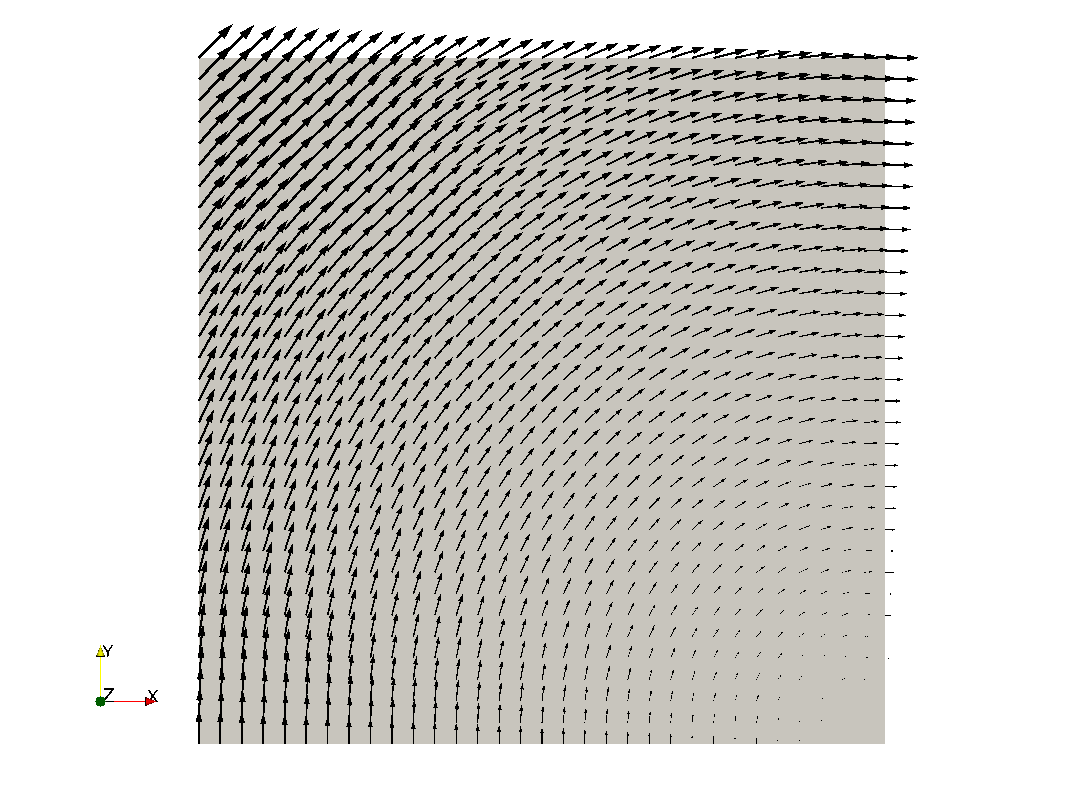
\includegraphics[height=4.cm]{python_codes/fieldstone_43/results/experiment5/vel}
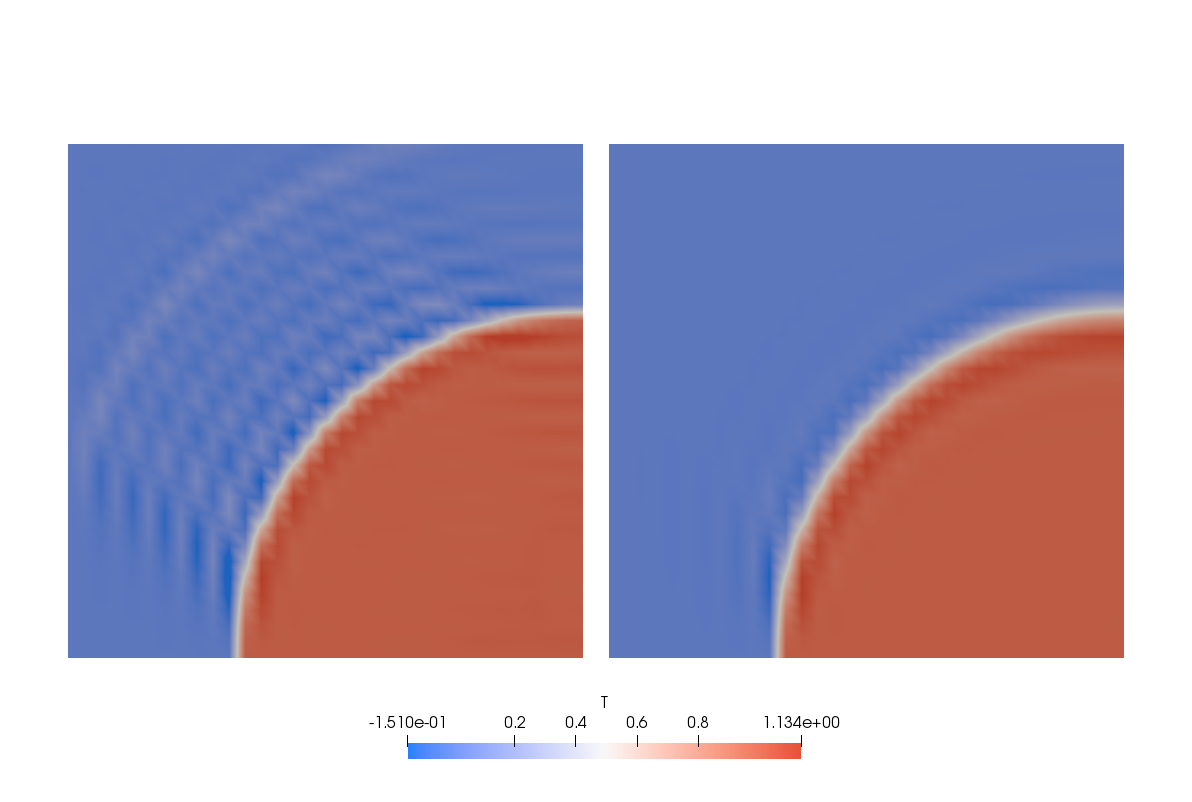
\includegraphics[height=4.cm]{python_codes/fieldstone_43/results/experiment5/T}
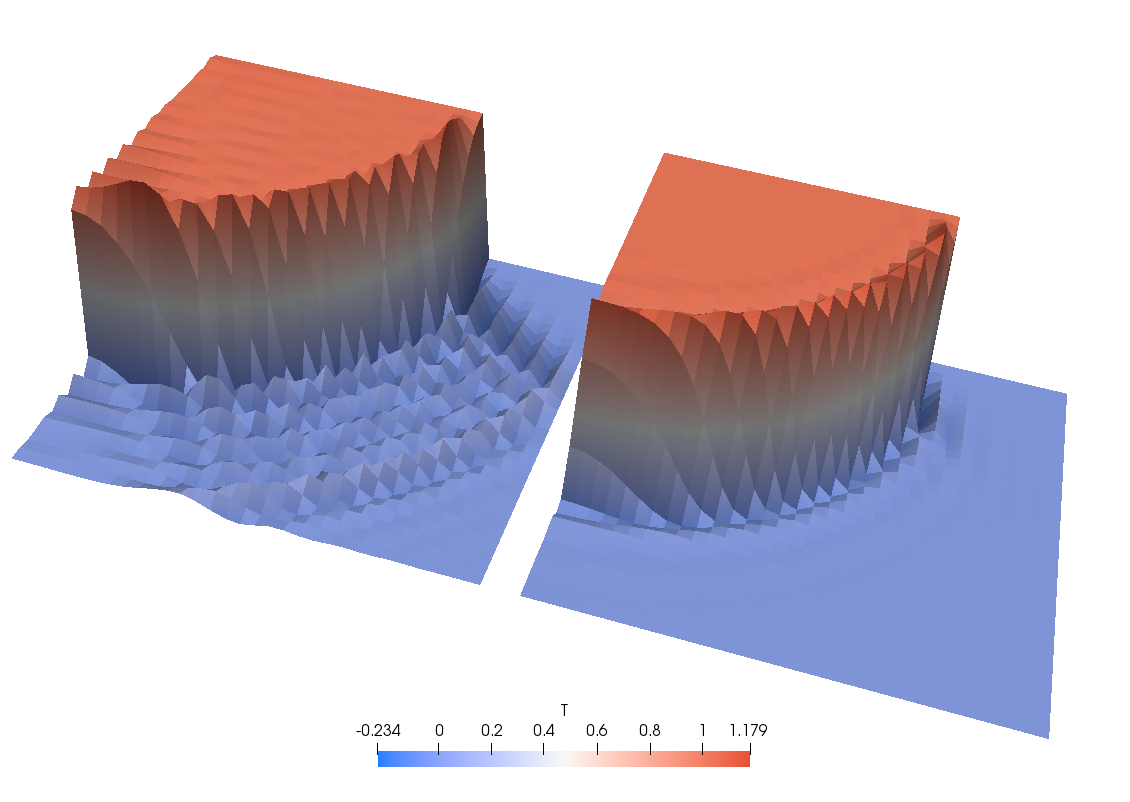
\includegraphics[height=4.cm]{python_codes/fieldstone_43/results/experiment5/T3D}\\
{\captionfont Left: no SUPG, Right: SUPG.}
\end{center}


\begin{center}
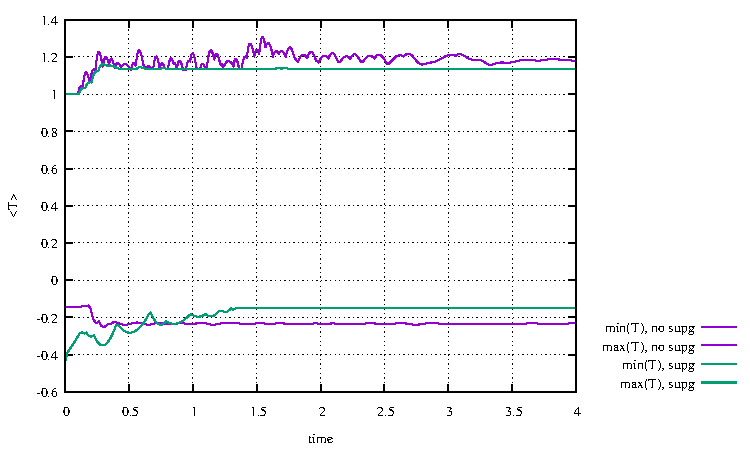
\includegraphics[width=7cm]{python_codes/fieldstone_43/results/experiment5/stats_T}
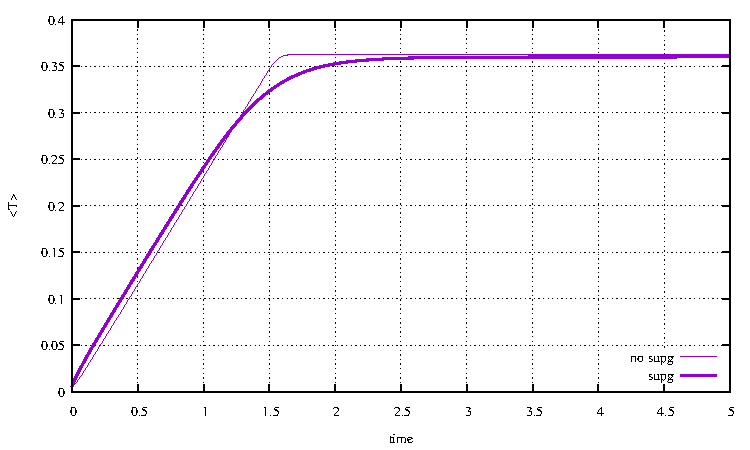
\includegraphics[width=7cm]{python_codes/fieldstone_43/results/experiment5/avrg_T}
\end{center}

Note that it is currently not possible to run this experiment with ASPECT.

%...........................................................................................
\paragraph{Experiment 6}

The domain is $1000\times1000$km, discretised with $50\times50$ elements. Boundary conditions are
$T=0$ on the top and bottom. On the left side $T=1$ if prescribed if $200<Y<800$km and 0 elsewhere.
The initial temperature field is a $800\times600$km square attached to the left.
The velocity is as follows and reaches a maximum on the right wall at 1cm/year:

\begin{center}
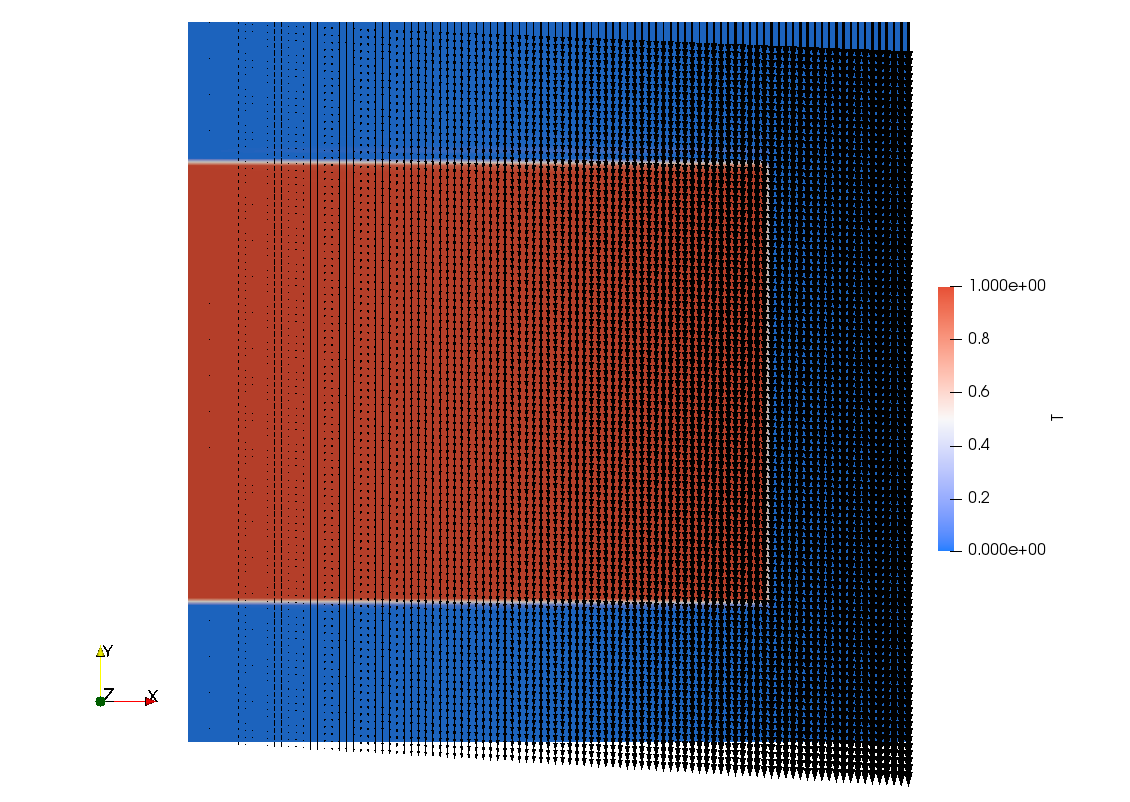
\includegraphics[width=7cm]{python_codes/fieldstone_43/results/experiment6/setup}
\end{center}

In this case, because of the very small velocity and the large size of the elements,  
the reported $\tau$ value is about $10^{13-15}$! 

\begin{center}
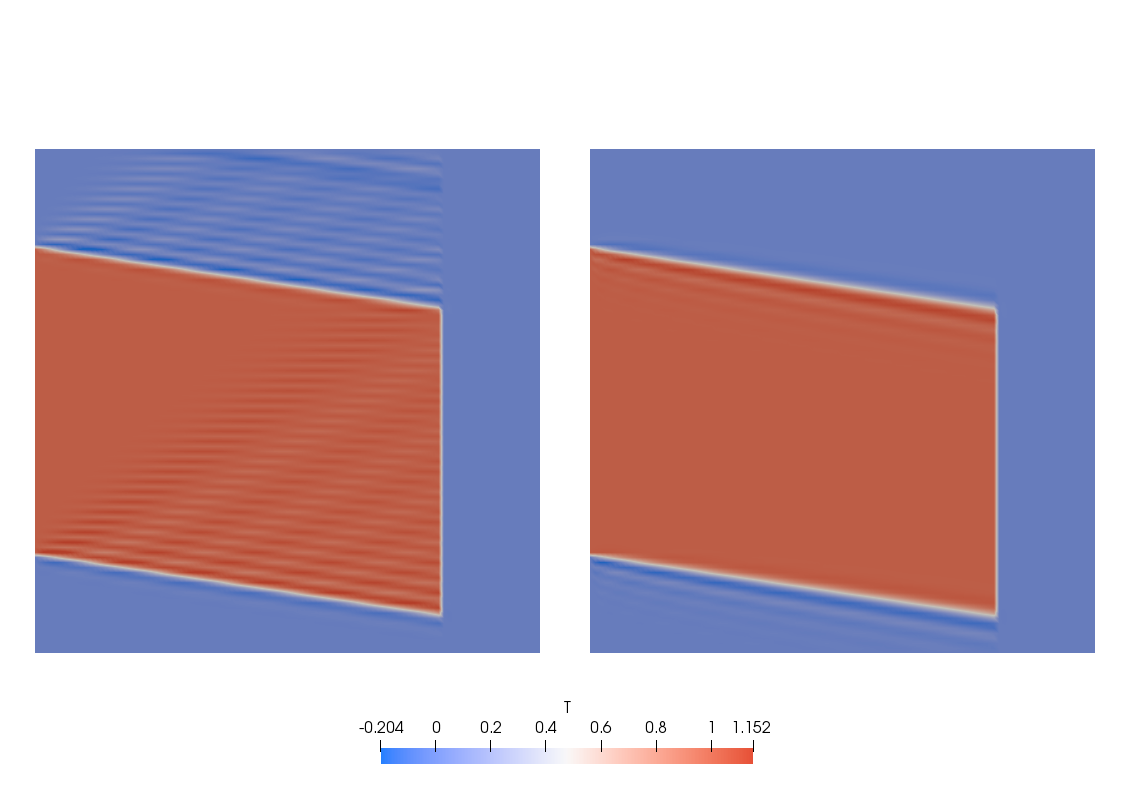
\includegraphics[width=14cm]{python_codes/fieldstone_43/results/experiment6/T}\\
{\captionfont Left: no SUPG; right: with SUPG}
\end{center}

Although SUPG removes the small wiggles, it does unfortunately not get rid of the 
large scale under/overshoots. 

\begin{center}
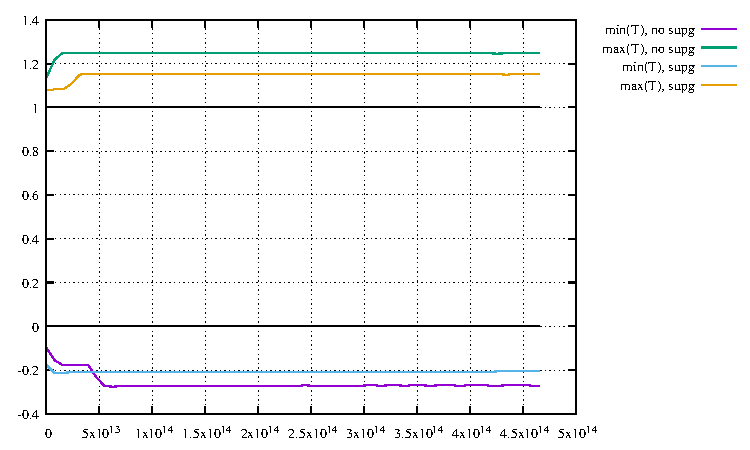
\includegraphics[width=7cm]{python_codes/fieldstone_43/results/experiment6/stats_T}
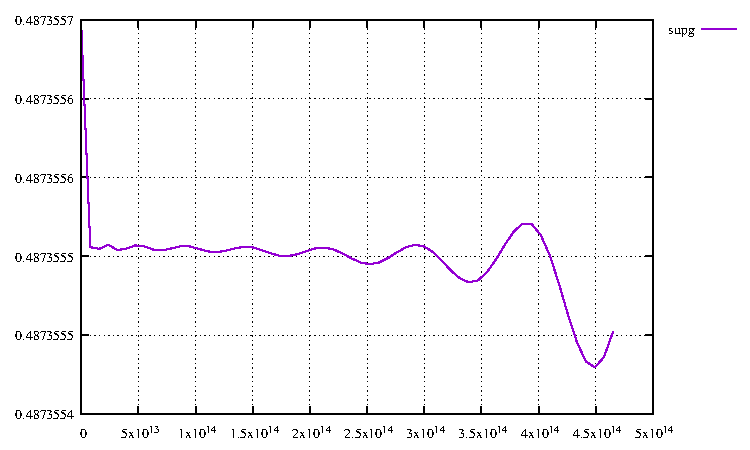
\includegraphics[width=7cm]{python_codes/fieldstone_43/results/experiment6/avrg_T}
\end{center}

%...........................................................................................
\paragraph{Experiment 7}

The setup is identical to experiment 6, but the velocity is now given by 
the equations of Section~\ref{mms1} which have been multiplied by 100 cm/year 
to arrive at a max velocity in the domain of approximately 1cm/year:

\begin{center}
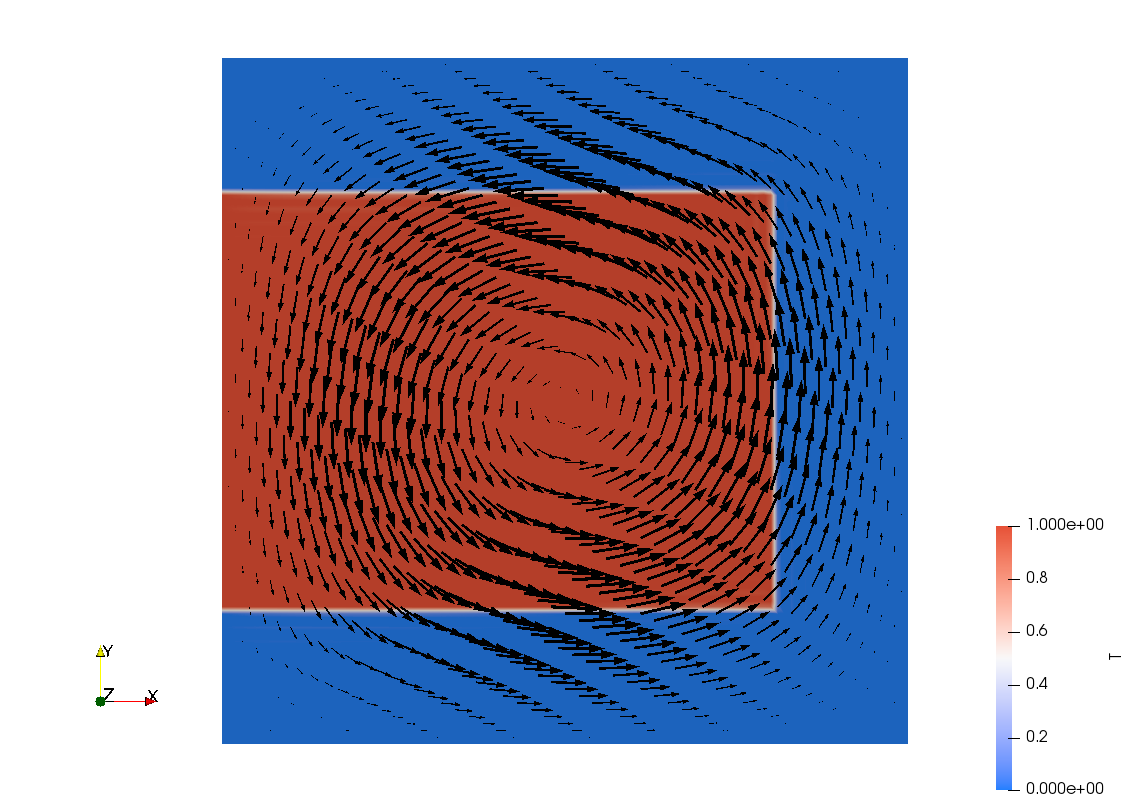
\includegraphics[width=7cm]{python_codes/fieldstone_43/results/experiment7/setup}
\end{center}

\begin{center}
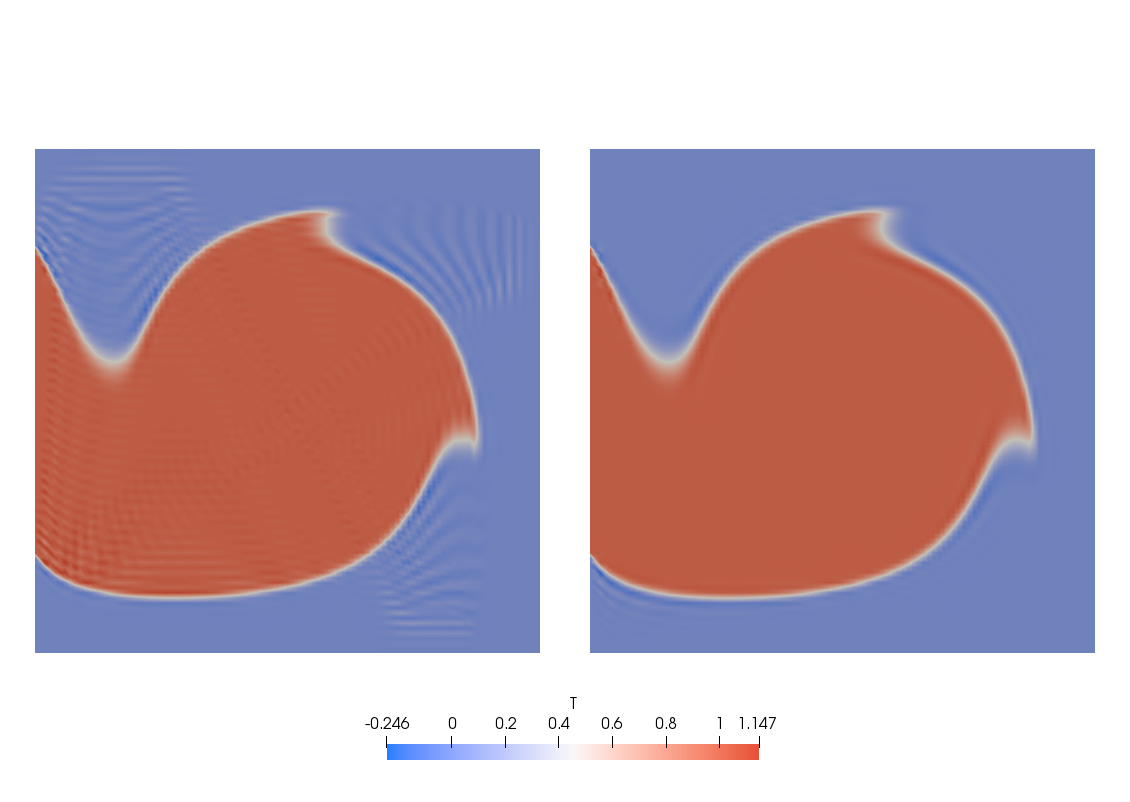
\includegraphics[width=14cm]{python_codes/fieldstone_43/results/experiment7/T}\\
{\captionfont Left: no SUPG; right: with SUPG}
\end{center}

\begin{center}
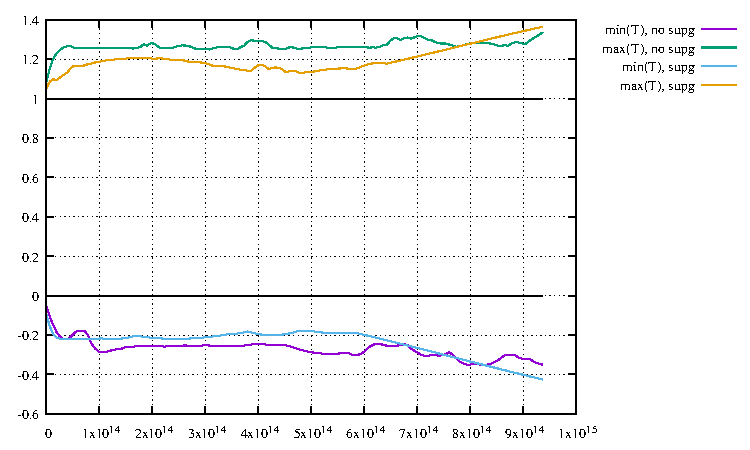
\includegraphics[width=7cm]{python_codes/fieldstone_43/results/experiment7/stats_T}
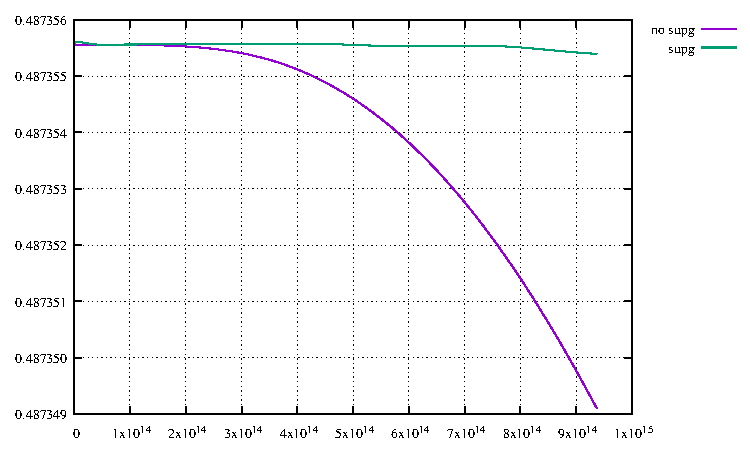
\includegraphics[width=7cm]{python_codes/fieldstone_43/results/experiment7/avrg_T}
\end{center}

Ripples are gone, but over/undershoots are about the same with and without supg ...?





